
\documentclass[journal]{IEEEtran} 

\pdfoutput=1

\usepackage[T1]{fontenc}
\usepackage[latin9]{inputenc}
\usepackage{verbatim}
\usepackage{float}
\usepackage{amsthm}
\usepackage{amsmath}
\usepackage{amssymb}
\usepackage{graphicx}
%\usepackage{multirow}
\usepackage{color}
\usepackage{url}


\newcommand{\TODO}[1]{{\color{red}{[#1]}}}

\makeatletter


%%%%%%%%%%%%%%%%%%%%%%%%%%%%%% Textclass specific LaTeX commands.
\numberwithin{equation}{section}
\numberwithin{figure}{section}
\theoremstyle{plain}
\newtheorem{thm}{\protect\theoremname}[section]
\theoremstyle{definition}
\newtheorem{defn}[thm]{\protect\definitionname}
\theoremstyle{remark}
\newtheorem{claim}[thm]{\protect\claimname}
\theoremstyle{plain}
\newtheorem{lem}[thm]{\protect\lemmaname}

\newtheorem*{lem*}{Lemma}
\theoremstyle{remark}
\newtheorem{rem}[thm]{\protect\remarkname}
\theoremstyle{plain}
\newtheorem{corollary}[thm]{\protect\corollaryname}
\theoremstyle{plain}
\newtheorem{proposition}[thm]{\protect\propositionname}
%%%%%%%%%%%%%%%%%%%%%%%%%%%%%% User specified LaTeX commands.

%\usepackage{babel}
\providecommand{\claimname}{Claim}
\providecommand{\definitionname}{Definition}
\providecommand{\lemmaname}{Lemma}
\providecommand{\remarkname}{Remark}
\providecommand{\theoremname}{Theorem}
\providecommand{\corollaryname}{Corollary}
\providecommand{\propositionname}{Proposition}


\newcommand{\RL}{\mathbb{R}^L}
\newcommand{\RN}{\mathbb{R}^N}
\newcommand{\CL}{\mathbb{C}^L}
\newcommand{\RNN}{\mathbb{R}^{N\times N}}
\newcommand{\CNN}{\mathbb{C}^{N\times N}}
\newcommand{\inner}[1]{\left\langle {#1} \right\rangle}
\newcommand{\E}[1]{\mathbb{E}\left\{{#1} \right\}}
\newcommand{\order}[1]{\mathcal{O}\left({#1} \right)}
\newcommand{\xz}{x_{\textrm{zp}}}
\newcommand{\DFT}[1]{\operatorname{DFT}\!\left( {#1} \right)}
\newcommand{\hx}{\hat{x}} 


\begin{document}

%\begin{frontmatter}


\title{Multireference alignment meets blind deconvolution}
\author{Tamir Bendory}
\maketitle

\begin{abstract}
	Here comes the abstract
\end{abstract}


\section{Introduction} \label{sec:introduction}

Blind deconvolution is the problem of estimating a signal from its convolution with an unknown kernel. This problem arises in many engineering and scientific applications, such as astronomy, communication, deblurring, acoustics, system identification and optics; see   \cite{jefferies1993restoration,tong1994blind,chan1998total,campisi2016blind,kundur1996blind,levin2011understanding,shalvi1990new,levin2009understanding,krishnan2011blind,ayers1988iterative,michaeli2014blind,lin2005relevant,abed1997blind}, just to name a few.

Without prior information, the blind deconvolution is clearly ill-posed. In this note, we consider a special case of the problem. We aim at estimating a signal $x\in\RL$ from $y\in\RN, \thinspace N\gg L$. The acquired data, the measurement $y$, is composed of many repetitions of $x$, at different positions, and i.i.d.\ normal noise $\varepsilon$ with mean zero and variance $\sigma^2$. 
Formally, our model read
\begin{equation}
y[n] = \sum_{i=1}^K \xz [n-n_i] + \varepsilon[n], 
\end{equation}
where $\xz\in\RN$ is a zero-padded version of $x\in\RL$  
defined as $$\xz  = [x, \underbrace{0,0,\ldots,0}_{N-L \text{ zeros}}],$$ and
 $n_i,\quad i=1,\ldots,K,$ are the translations of $\xz$.


Note that both $x$ and the translations, or positions, $n_i$ are unknown. Let $s\in\{0,1\}^N$ be the ``support" signal, which takes the value 1 at the locations $n_i$ are zero otherwise. 
Then, 
\begin{equation}
y = \xz \ast s + \varepsilon.
\end{equation}
The goal is then to estimate $x$ from $y$, while $s$ is unknown as well. The support signal $s$ is the latent or hidden variable of the problem. The situation where both signals are unknown, but the goal is merely estimating one of them  is quite common situation in blind deconvolution problem. For instance, in image deblurring, both the blurring kernel and the high-resolution image are unknown, but the main goal is merely to sharpen the image. In Section~\ref{sec:literature} we survey previous results on blind deconvolution.

Figure~\ref{fig:example} shows examples of the problemin different noise levels. In the low noise regime (for instance, the first row), the problem is rather easy. In this case, one can identify $x$ in $y$ by simple detection algorithms (e.g., thresholding on the correlation function). Once several copies of the signal were detected and cropped from $y$, then one can  improve the SNR by averaging. We are interest in the more challenging regime of high noise level, in which the signal is completely swamped in the noise, and one cannot detect the signal's appearances. In this case, one need to use the prior information that the signal appears many times across the measurement.

\begin{figure*}
	\begin{center}
	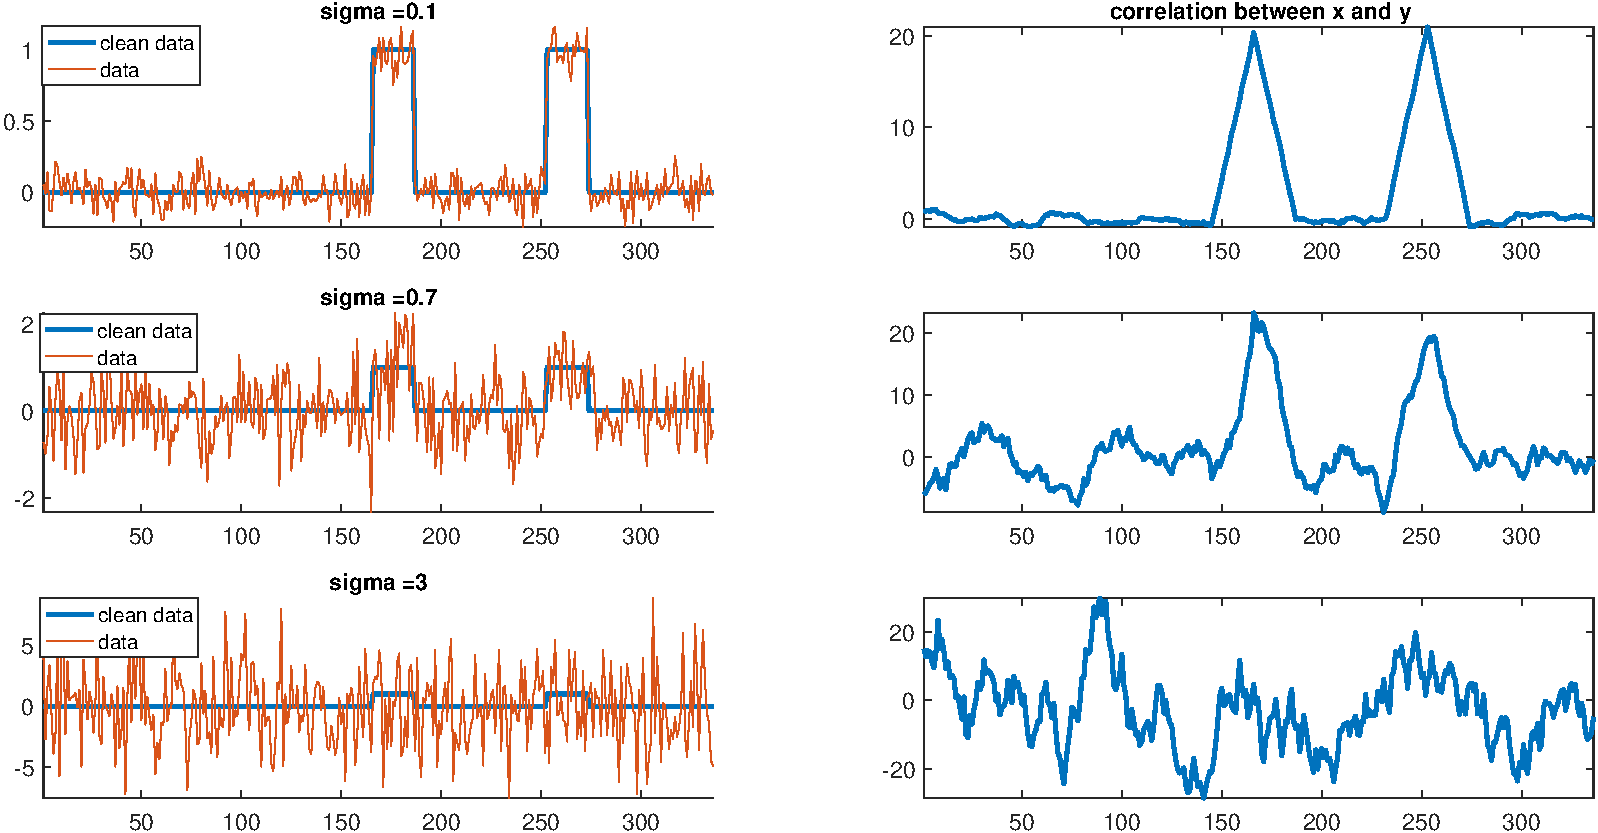
\includegraphics[scale = .5]{example}
	\end{center}
\caption{The left column presents the clean data and the measurement in different noise levels. In this example, a signal of length $L=21$ appears twice in a measurement of length $N=336$ with different noise levels. Note to the different scale of the y-axis. The right column presents the correlation between the signal and the measurement for the associated problems. }
\label{fig:example}
\end{figure*}

Our approach for this blind deconvolution problem utilized  tools recently that were developed for the multireference alignment problem. Multireference alignment (MRA) is the problem of estimating a signal from its circularly-shifted noisy measurements~\cite{bandeira2014multireference,bendory2017bispectrum}. In Section~\ref{sec:mra}, we survey recent works in this field and its relation with our problem. Particularly, we use the method proposed in~\cite{bendory2017bispectrum} of invariant features. In short, the idea is to split $y$ into a bunch of shorter windows. If each window contains exactly  one signal, then the problem reduces exactly the MRA problem. However, this is not the case. Some windows contain only noise, while others contain both noise and parts of a signal. In Section~\ref{sec:algorithm} we present and discuss the algorithm. 

The outline of this paper is as follows. In Section~\ref{sec:literature} we introduce the background of relevant papers for this work. Particularly, in Section~\ref{sec:blind_deconvolution} we discuss the blind deconvolution problem and in Section~\ref{sec:mra} we introduce and survey the MRA problem. In Section~\ref{sec:cryoEM} we introduce the mathematical formulation of the cryo--electron microscopy (EM) imaging technique. The model we consider in this note can be viewed as a simplified model for the cryo--EM problem as will be explained. In Section~\ref{sec:algorithm} we introduce of algorithm and analyze it in Section~\ref{sec:analysis}. Section~\ref{sec:experiments} is devoted for numerical experiments. Section~\ref{sec:conclusion} concludes the manuscript.
 



\section{background and literature survey} \label{sec:literature}

In this section, we introduce the two main ingredients of this work, blind deconvolution and MRA.

\subsection{Blind deconvolution} \label{sec:blind_deconvolution}


Blind deconvolution is the problem of recovering a signal from its convolution with unknown kernel. That is, recovery of $x$ from
\begin{equation}
y = x\ast k,
\end{equation}
where both $x$ and $k$ are unknown. In the Fourier domain, it takes the form of 
\begin{equation}
Fy = Fx \odot Fk,
\end{equation}
where $Fz$ stands for the Fourier transform of $z$.

Clearly, without prior information of the signal, it is impossible to estimate the signal. The problem has been analyzed recently with a various convex and non-convex algorithms under the assumption that the signal is in a known  subspace spanned by vectors with random entries~\cite{ahmed2014blind,li2016rapid,ling2017blind} 
and under sparsity in a random linear subspaces~\cite{lee2017blind,li2016identifiability,kech2017optimal,ling2015self,chi2016guaranteed,li2015unified}. 

We briefly mention that the deconvolution problem, namely, when the kernel is assumed to be known, has been analyzed throughly in recent years under sparsity constraints~\cite{bendory2016robust,bendory2017robust,bendory2016stable,boyer2017adapting,bernstein2017deconvolution,de2012exact,azais2015spike,duval2015exact,duval2015sparse}.  Nonetheless, the problem under consideration is essentially different. From two reasons. First, of course, we consider the blind setting when the kernel is unknown. Second, these works considered the recovery of sparse signal, with Gaussian-like kernel. In our problem, the convolution kernel is sparse, and we aim to recover a general signal. 

As far as we know, no work considered the blind deconvolution considered in this manuscript. In~\cite{choudhary2014sparse}, it  was shown that 
a simple sparsity assumption in the canonical basis is insufficient
for unique recovery. However, here we also assume that the sparse signal is binary. In addition, we mainly care of the problem in the high noise regime and understanding how the relations between the parameters of the data effects the estimation error. 


\subsection{Multireference alignment} \label{sec:mra}


Multireference alignment is the problem of estimating a signal $x\in\RL$ from its circularly shifted noisy measurements
\begin{equation} \label{eq:mra}
y_j = R_{r_j}x + \varepsilon_j, \quad j = 1,\ldots,N
\end{equation}
where $R_{r}$ translates a signal by $r$ locations, namely, $(R_rx)[i] = x[i-r]$, and $\varepsilon$ is an i.i.d.\ normal noise with mean zero and variance $\sigma^2$. This problem has application in radar, image processing and structural biology~\cite{zwart2003fast,foroosh2002extension,diamond1992multiple}. The algorithmic and statistical characterizations of this problem have been analyzed thoroughly in the last couple of years, see~\cite{bendory2017bispectrum,bandeira2014multireference,bandeira2017optimal,perry2017sample,boumal2017heterogeneous,abbe2017multireference,abbe2017sample}.

In this work, we exploit the framework proposed in~\cite{bendory2017bispectrum}. The idea is to use features of the signal that are invariant under translation. Specifically, it was proposed to estimate the mean, power spectrum and bispectrum of the signal from the data. The estimation is performed by averaging over the features of the measurements. Let $\mu_z,P_z$ and $B_z$ denote the mean, power spectrum and bispectrum of a signal $z$. Then, it can be shown that 
\begin{align}
\frac{1}{N}\sum_{i=1}^N\mu_{y_j}  &\,\to \, \mu_x, \\
\frac{1}{N}\sum_{i=1}^NP_{y_j}  &\,\to \, P_x + L\sigma^2, \\
\frac{1}{N}\sum_{i=1}^NB_{y_j}  &\,\to \, B_x + \mu_x\sigma^2L^2A, 
\end{align} 
where $A$ is a known deterministic matrix. Therefore, by proper debiasing, one can get a reliable estimating of these features. For $\sigma,N\to\infty$, the estimation rate is dominated by the bispectrum and thus the estimation rate is $\sigma^6/N$, which is optimal for uniform distribution of translations~\cite{bandeira2017optimal}. Given reliable estimation of the features, the signal can be accurately estimated, up to translation, using a variety of algorithms~\cite{bendory2017bispectrum}.




\subsection{Connection with the cryo--EM problem} \label{sec:cryoEM}

This work is partially motivated by the imaging
technique called single particle Cryo--EM, enabling the visualization of molecules at near atomic resolution~\cite{bartesaghi20152,sirohi20163}. In cryo--EM, many samples of a molecule are frozen in a thin sheet of ice. Then, the microscope transmits electrons and we acquire  several images, called \emph{micrographs}, that contains the two-dimensional tomographic projections of the samples. The  cryo--EM 
problem is then to estimate the molecules from several micrographs. 

\begin{figure}
	\begin{center}
		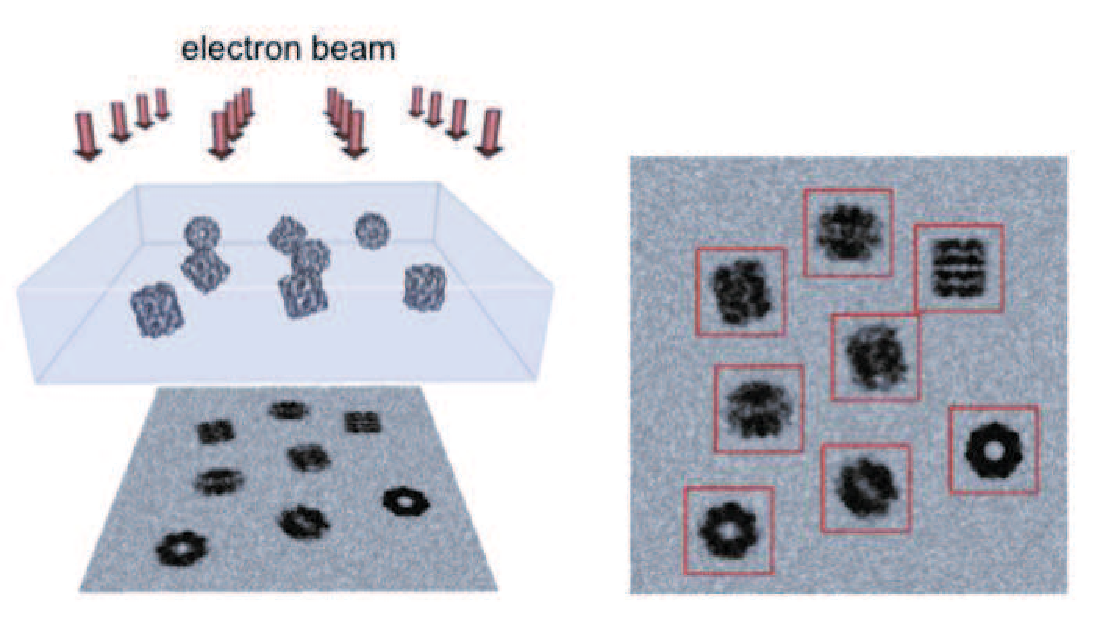
\includegraphics[scale = .4]{cryoem-eps-converted-to}
	\end{center}
	\caption{A schematic draw of the micrograph generation. Courtesy of ?}
	\label{fig:cryo-EM}
\end{figure}

\begin{figure}
	\begin{center}
		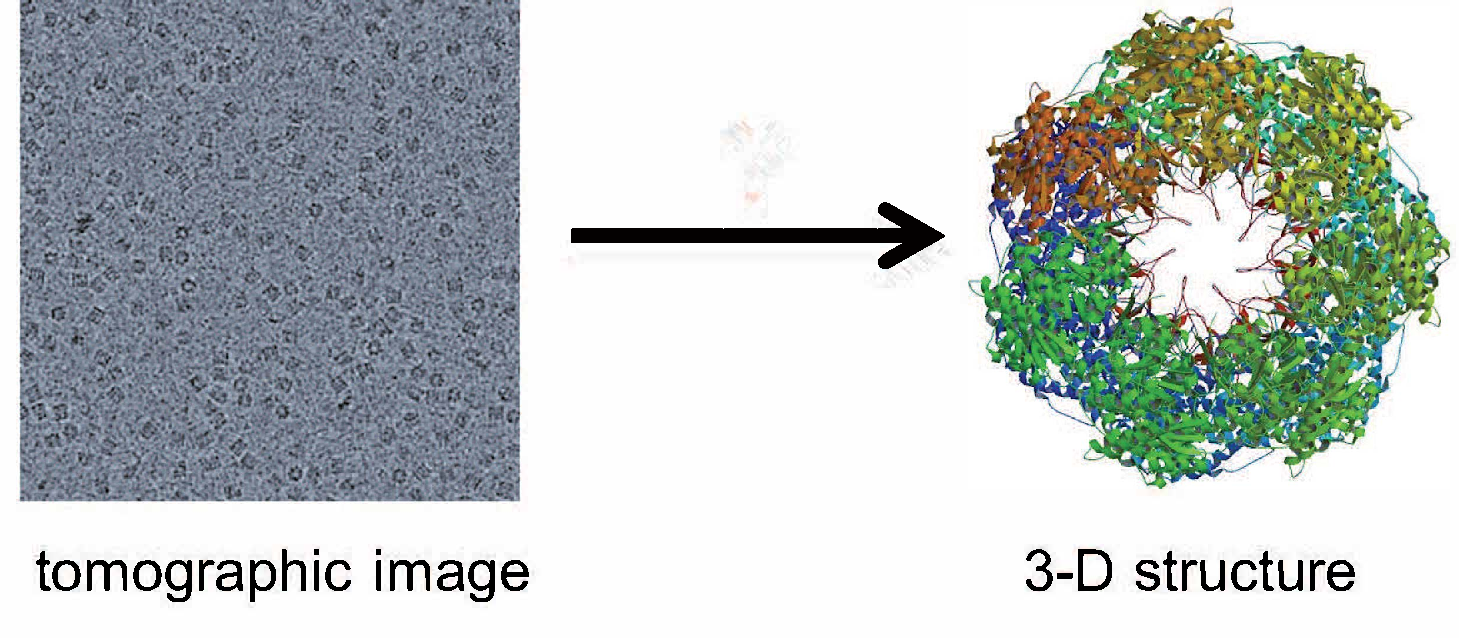
\includegraphics[scale = .35]{cryoem-problem-eps-converted-to}		
	\end{center}
	\caption{The cryo--EM problem: estimating a molecule from the micrograph. Courtesy of ?}
	\label{fig:cryo-EM-problem}
\end{figure}

A standard cryo--EM reconstruction algorithm starts with a stage called \emph{particle picking} [ref]. In this stage, the projections are detected in the micrographs, and then cropped. Then, ideally, one get a set of measurements of the form 
\begin{equation} \label{eq:cryo-em}
y_j = \mathcal{P}( g_j\circ x) + \varepsilon_j,\quad j=1,\ldots,N, 
\end{equation}
where $x$ is the three-dimensional molecule to be estimated,  $g_j\in SO(3)$ are unknown 3D rotations that act on the molecule and $\mathcal{P}$ is a tomographic projection. This model has been analyzed theoretically from different point--of-views~\cite{bandeira2015non,hadani2011representation} [more ref]. The MRA model~\ref{eq:mra} can be interpreted as a simplification of the cryo--EM problem, where the unknown shifts correspond to the unknown rotations (but there is no analog for the projection operation).

In practice, particle picking algorithms are far from being optimal. For instance, the projections in the cropped images are not centered, and therefore an unknown  two-dimensional translation should be added to the model~\eqref{eq:cryo-em}. In addition, most of the particle picking algorithms throw away many particles since they fail to detect them. Hence, a necessary condition for the success of such algorithm is that the noise level would low enough so that detection would be possible.

Our work can be viewed as a first stage towards answering the question whether molecule estimation is possible in a very low SNR regime, where \emph{detection is impossible}. Our model can be seen as a very simplified cryo--EM model, where $y$ corresponds to the micrograph and the signal repeated signal $x$ to the molecule. The success to estimate the signal in the very low SNR regime may indicate that the molecule can be estimated directly from the cryo--EM micrographs, even if the SNR is so low that particle picking fails. 

   

\section{Algorithm} \label{sec:algorithm}


Before moving ahead to the feature estimators, we need to estimate the norm of the signal. This is necessary since many analysis windows do not contain information on the signal, but pure noise. We will use the norm to scale the the signal's estimator.
This can be done as follows. For short, we denote $x_K[n]=\sum_{i=1}^K \xz[n-n_i]$ and note that $\|x_K\|_2^2 = K\|x\|_2^2$. 
Then,
\begin{equation}
\| y\|_2^2 =  \| x_K\|_2^2 + \|\varepsilon\|_2^2 + 2\varepsilon^Tx_K. 
\end{equation}  
As $N\to\infty$, we can estimate 
\begin{equation}
\begin{split}
\E{\| y\|_2^2} &=  \| x_K\|_2^2 + \E{\|\varepsilon\|_2^2} + 2\E{\varepsilon^Tx_K} \\ 
&= K\|x\|_2^2 + N\sigma^2. 
\end{split}	 
\end{equation}   
And therefore, 
\begin{equation}
\|x\|_2^2 \approxeq \frac{\| y\|_2^2 - N\sigma^2}{K}. 
\end{equation}




To perform this blind deconvolution, we use the invariant approach proposed for multireference alignment in a previous paper. Let us  first introduce  notation. We crop the measurement $y\in\RN$ into a series of analysis windows: 
\begin{equation}
y_i = y[(i-1)W + 1 : iW ]\in\mathbb{R}^W, \quad i=1,\ldots,N/W, 
\end{equation}
To ease notation, we assume that  $W$ divides $N$  so that there are exactly $N/W$ windows. We also assume that $\vert n_i - n_j\vert >W$ so that each window contains no more than one signal (in general, we can introduce overlapping windows. The code enables it, but it does not seem to improve performance.).
For each one of the windows, we compute its first three translation-invariant features, namely, mean, power spectrum and bispectrum. We then hope that averaging over these features will produce a reliable estimation of the invariant features of the signal itself. 
We recall that given accurate estimators of those features, we can estimate the signal itself reliably. Therefore, the question boils down to the accuracy of these feature estimations.

\section{Analysis} \label{sec:analysis}


Next, we analyze the feature estimation in the asymptotic regime of $N,\sigma,K\to\infty$ and fixed $L,W$. We introduce the ``sparsity factor" defined as $S = \frac{N}{WK}<\infty$, $WK$ is a measure for the ``active" windows. We also define  another zero padded signal $x_W  = [x, \underbrace{0,0,\ldots,0}_{N-W \text{ zeros}}]\in\mathbb{R}^W$.

We want to estimate the features of this signal, and focus on the bispectrum for the sake of simplicity (the estimation of the power spectrum and mean obeys the same methodology). 
In order to estimate the bispectrum we average over the bispectra of the windows, namely, (for the power spectrum, we need to do unbiasing. In addition, we can replace the mean by more robust estimator, like the median.)
\begin{eqnarray}
\hat{B}_{x_W} = \frac{W}{N}\sum_{i=1}^{N/W}B_{y_i}.
\end{eqnarray}
We split the sum into three groups of the windows:
\begin{eqnarray}
\hat{B}_{x_W} = B_\textrm{signal} + B_\textrm{clutter} + B_\textrm{noise}, 
\end{eqnarray}
where
\begin{itemize}
	\item $B_\textrm{noise}$ - sum of the bispectra of the segments that contain pure noise (no signal),
	\item $B_\textrm{signal}$ - sum of the bispectra of the segments that contain a full signal (one appearance of $x$) and noise,
	\item $B_\textrm{clutter}$ - sum of the bispectra of the segments that contain only part of $x$ and noise.
\end{itemize}

We first observe that $B_\textrm{noise}\to 0$ (note that this is the zero matrix). More precisely, the variance of the noise goes to zero at rate  $\order{\frac{W}{N}\left(1-\frac{1}{S}\right)\sigma^6}$. In addition, under the assumption that $n_i$ (if appear) are distributed uniformly in the window (we need to come up with precise statistical model; but it would be rather easy), there are (asymptotically) $K(1-L/W)$ windows with complete signals. Therefore,
$B_\textrm{signal}\to \frac{KW(1-L/W)}{N}B_x$ at rate $\order{\frac{\sigma^6}{K(1-L/W)}}$. (Here we need to be a bit careful with the mean of the signal, or to assume it is zero.) Note that the scaling would be corrected at the last stage of the algorithm, by rescaling according to the estimated  norm.

The more interesting term is the ``clutter" --- the cropped signals. Since each such signal appears in two windows,
we have $2KL/W$ clutter segments. Of course, the noise in this segments goes to zero
at rate $\order{\frac{W\sigma^6}{2KL}}$. However, we have an additional error term arises from  the cropped signals. To analyze the effect of this term, let us assume that $N/\sigma^6$ is great enough so that $B_\textrm{noise}\to 0$. Then,
\begin{equation}
\begin{split}
\left\| \hat{B}_{x_W} - B_\textrm{signal}\right\|_{\textrm{F}} \approxeq&  \left\|B_\textrm{clutter}\right\|_{\textrm{F}}
= \left\|\frac{W}{N}\sum_{i\in\textrm{clutter}}B_{y_i}\right\|_{\textrm{F}}
\\ \leq & 
\frac{W}{N}\frac{2KL}{W}\left\|B_x\right\|_{\textrm{F}} = \frac{2L}{SW}
\|B_x\|_{\textrm{F}}.
\end{split}
\end{equation}
Therefore, for large sparsity term $S$ or large $W/L$, we get an accurate estimation of a scaled version of the signal's bispectrum. 


Few insights from the analysis: (need to check numerically)
\begin{itemize}
	\item Larger $S$ reduces the clutter error, however, increases the variance of the noise estimation.
	\item Larger $W/L$ reduces the clutter error, however, increases the variance of the noise  of $B_\textrm{noise}$.
	\item We must keep $W/L$ large enough to see enough full signals.    
\end{itemize} 


\section{Numerical experiments} \label{sec:experiments}

\section{Conclusion} \label{sec:conclusion}




\bibliographystyle{plain}
\bibliography{ref}

\end{document}


 